\chapter{Introduction}
\label{sec:Introduction}

Provide a general introduction to what the thesis is all about. Here you present the question or problem you aim to answer or address with your thesis, some of the reasons why it is a worthwhile topic, your motivation for answering this question/solving this problem, the contribution of your work and an overview of your main results. 

\begin{itemize}
    \item 1 paragraph introduction of study context;
    \item 1 paragraph what has been done in prior work and where the gap is that the thesis addresses
    \item 1 paragraph research questions
    \item 1 paragraph study design overview
    \item 1 paragraph findings overview and implications
\end{itemize}

Useful examples below:
This is an example of a citation \cite{einstein}.

This is an example how to add a Figure \ref{fig:plot}:
\begin{figure}[htb]
\centerline{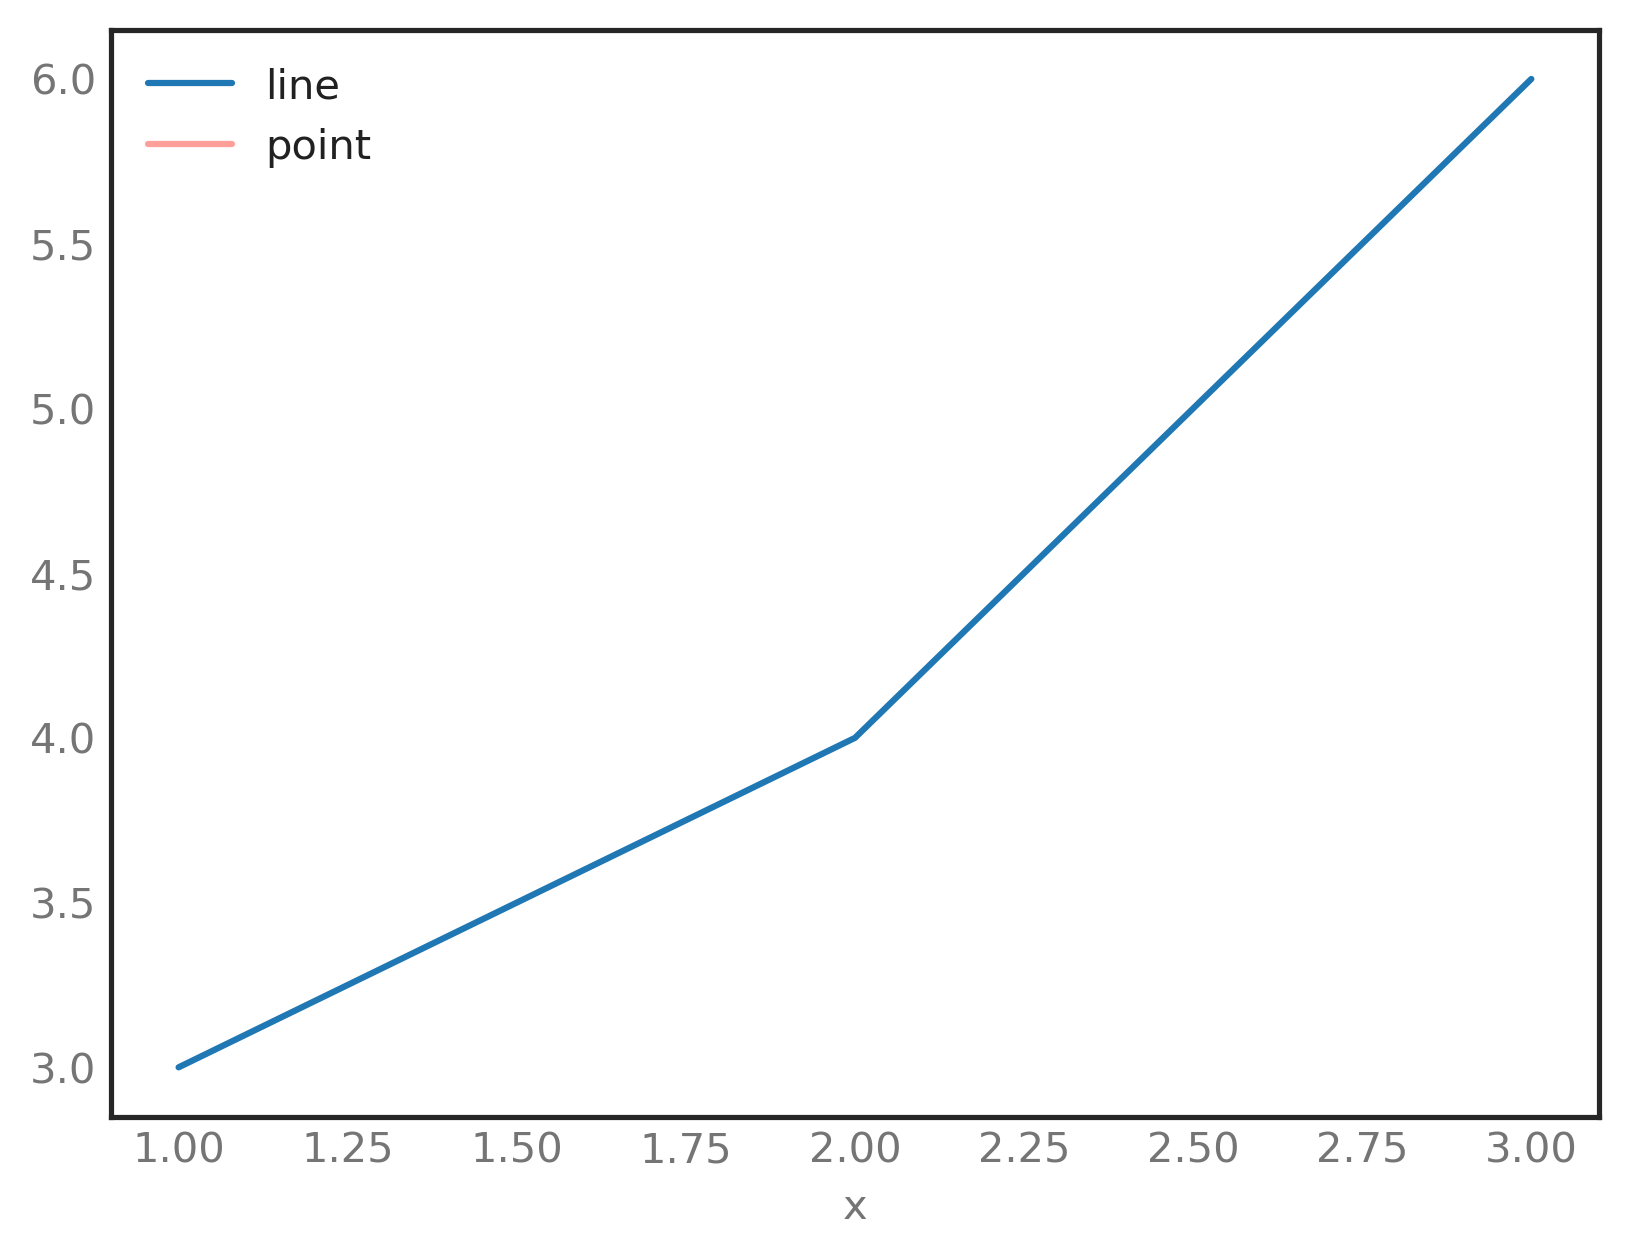
\includegraphics[width=13cm,keepaspectratio,]{images/plot-example.png}}
\caption{Example of a random plot}
\label{fig:plot}
\end{figure}

An example of a Table \ref{tab:regr}
\begin{table}[h]
\begin{center}

\begin{tabular}{L{2.5cm}L{2cm}L{2cm}L{2cm}L{2cm}}
\toprule 
Descriptives       & Mean & Standard Deviation & Minimum & Maximum \\ \hline
Team size               & 3.28      & 1.05   & 2              & 8             \\
Technical complexity & 4.82      & 3.02                & 1             & 18             \\
Winning      & 0.21     & 0.32                & 0             & 0.9            \\
Skill diversity         &  0.51     &  0.18               & 0              & 0.8            \\
Skill matching         & 0.25      & 0.22             & 0             & 1             \\
Team familiarity         & 0.08      & 0.3           & 0            & 3            \\
Preparation             & 0.25      & 0.43                & 0             & 1            \\
Hackathon experience      & 1.73     & 1.31           & 0.5             & 17            \\
Continuation intentions      & 0.60     & 0.49           & 0             & 1            \\ \bottomrule
\end{tabular}
\end{center}

\caption{Example Table.}
\label{tab:regr}
\end{table}